\usetikzlibrary{calc}

\tikzset{
% Two node styles for game trees: solid and hollow
solid node/.style={circle,draw,inner sep=1.5,fill=black},
hollow node/.style={circle,draw,inner sep=1.5},
square node/.style={rectangle,draw, inner sep = 1, fill = black}
}

% Specify spacing for each level of the tree
%\tikzstyle{level 1}=[level distance=12mm,sibling distance=15mm]
%\tikzstyle{level 2}=[level distance=15mm,sibling distance=15mm]
%\tikzstyle{level 3}=[level distance=13mm,sibling distance=11mm]


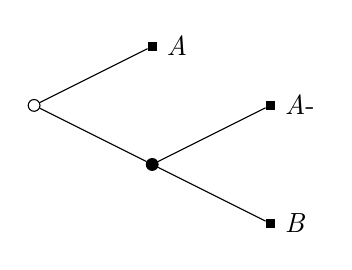
\begin{tikzpicture}[grow=right, sloped]
\node[hollow node, draw] {}
    child {
        node[solid node, draw] {}
        child {
            node[square node, fill, inner sep=1.5pt, label=right:{\emph{B}}] {}
            edge from parent
            node[above] {}
        }
        child {
            node[square node, fill, inner sep=1.5pt, label=right:{\emph{A}-}] {}
            edge from parent
            node[below] {}
        }
        edge from parent
        node[below] {}
    }
        child {
        node[square node, fill, inner sep=1.5pt, label=right:{\emph{A}}] {}
        edge from parent
        node[above] {}
    };
\end{tikzpicture}
